\documentclass[border=0.1cm]{standalone}
\usepackage{tikz}

\begin{document}
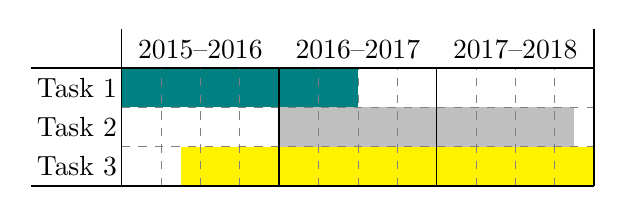
\begin{tikzpicture}
% Coloring ..
\path[fill=teal](0,1) rectangle (3,1.5);
%\draw[fill=teal,ultra thin] (0.001,1.001) rectangle (2.999,1.499); % Task one

\path[fill=lightgray] (2,0.5) rectangle (5.75,1);
%\draw[fill=teal,ultra thin] (2.001,0.501) rectangle (5.499,0.999); % Task two

\path[fill=yellow] (0.75,0) rectangle (6,0.5); % Task three

% Writing
\node [align=center,right] at (-1.2,1.25) {Task 1}; % Tasks
\node [align=center,right] at (-1.2,0.75) {Task 2};
\node [align=center,right] at (-1.2,0.25) {Task 3};
\node [above] at (1,1.5) {2015--2016}; % Years
\node [above] at (3,1.5) {2016--2017}; 
\node [above] at (5,1.5) {2017--2018}; 

% creating axis
\draw[help lines,dashed,ystep=0.5,xstep=0.5] (0,0) grid (6,1.5);
\draw[semithick](0,0) -- (0,2); % Vertical
\draw[semithick](2,0) -- (2,1.5);
\draw[semithick](4,0) -- (4,1.5);
\draw[semithick](6,0) -- (6,2);
\draw[semithick](-1.15,1.5) -- (6,1.5); % Horizontal
%\draw[thick](0,1) -- (6,1);
\draw[semithick](-1.15,0) -- (6,0);
\end{tikzpicture}
\end{document}